\documentclass[11pt]{article}
\usepackage[margin=1in,letterpaper]{geometry}
\usepackage{amsmath,amssymb,amsthm,graphicx}
\usepackage[colorlinks=true,linkcolor=blue!45!black,citecolor=blue!45!black,urlcolor=blue!45!black]{hyperref}
\usepackage{xcolor}
\usepackage{microtype}
\hypersetup{pdftitle={Two Euler factors in a smoothed prime sum},pdfauthor={},pdfsubject={Exact local corrections, their limiting laws and a Riemann hypothesis criterion}}
\setlength{\parindent}{1.3em}
\setlength{\parskip}{0pt}
\raggedbottom
\newtheorem{theorem}{Theorem}[section]
\newtheorem{prop}[theorem]{Proposition}
\newtheorem{cor}[theorem]{Corollary}
\newcommand{\T}{\mathbb T}
\newcommand{\Prob}{\mathbb P}
\newcommand{\E}{\mathbb E}
\newcommand{\dd}{\,\mathrm d}
\DeclareMathOperator{\Law}{Law}
\newcommand{\RR}{\mathbb R}
\numberwithin{equation}{section}
\title{\bfseries Two Euler factors in a smoothed prime sum}
\author{}
\date{\normalsize November 21, 2026}
\begin{document}
\maketitle
\begin{abstract}
Removing the powers of two distinct primes from the von Mangoldt sum
with weight $(x/n-1)_+$ leaves a bounded oscillation after the linear
and logarithmic terms are subtracted. We compute its distribution under
logarithmic averaging. If $s$ is the distance from an endpoint of its
support, the lower tail is asymptotic to a constant times $s$, whereas
the upper tail is asymptotic to a constant times $s^2$. We determine
both constants. Under uniform sampling of the integers there is a
family of subsequential laws indexed by a two-dimensional torus.
For the eight reduced classes modulo $24$ we use the classical explicit
formula to express the Riemann hypothesis as a sharp uniform bound
on the remaining prime sum. Along the integers its normalized upper
limit is exactly $2+\gamma-\log(4\pi)$ under RH and infinite if RH fails.
\end{abstract}
\section{Deleting two primes}\label{sec:local}
The eight reduced residue classes modulo $24$ are
$1,5,7,11,13,17,19,23$. Plichta's prime cross draws these classes
as spokes of a wheel. Grant and Ghannam use the same picture
\cite{plichta,grant}. A prime greater than $3$ lies on one of these
spokes, as does a composite such as $91$. For the von Mangoldt function
$\Lambda$, which takes the value $\log p$ on $p^k$, $k\geq1$, and is
zero elsewhere, restricting to these eight classes has a precise effect.
It removes only the powers of $2$ and $3$.

We consider a weight used by Alpöge \cite[p.~3, item 5]{alpoge}.
For $x\geq1$ real and $m\geq1$ an integer, define
\begin{align}
 S_m(x)&=\sum_{\substack{n\leq x\\(n,m)=1}}\Lambda(n)(x/n-1),
 &c_m&=\sum_{p\mid m}\frac{\log p}{p-1},\notag\\
 E_m(x)&=S_m(x)-x\log x+(1+\gamma+c_m)x. \label{eq:normalization}
\end{align}
Here $\gamma$ is Euler's constant. Write $E=E_1$, $\ell_p=\log p$
and $a_p=\ell_p/(p-1)$. For $0\leq v\leq1$ define
\[
 f_p(v)=a_p e^{\ell_p v}-\ell_p v.
\]
Since $f_p(0)=f_p(1)=a_p$, this gives a continuous function on the
circle $\T=\RR/\mathbb Z$. All measures on tori below are normalized
Lebesgue measures. We use natural logarithms throughout.

\begin{prop}[Exact correction]\label{prop:local}
For every $m\geq1$ and $x\geq1$,
\begin{equation}
 E_m(x)=E(x)+\omega(m)\log x+
 \sum_{p\mid m}f_p\!\left(\frac{\log x}{\ell_p}\right),
 \label{eq:correction}
\end{equation}
where $\omega(m)$ is the number of distinct prime divisors of $m$.
\end{prop}
\begin{proof}
For a prime $p\mid m$ put $K=\lfloor\log x/\ell_p\rfloor$ and
$u=x/p^K$. The contribution of its deleted powers to $S_1-S_m$ is
\[
 \ell_p\sum_{k=1}^K(xp^{-k}-1)
 =a_p(x-u)-K\ell_p.
\]
The normalization restores $a_px$, and
$K\ell_p=\log x-\log u$.
The remaining term $a_pu-\log u$ is exactly
$f_p(\log x/\ell_p)$. Distinct primes have disjoint sets of positive
powers. At $x=p^K$ the last summand vanishes, so the formula includes
every endpoint.
\end{proof}

For the rest of the distributional analysis fix distinct primes $p,q$.
Set $\omega=(1/\ell_p,1/\ell_q)$,
$F(v,w)=f_p(v)+f_q(w)$, and $R_{p,q}(x)=F(\omega\log x)$.
Write $R_{24}=R_{2,3}$. Logarithmic oscillations in sums over geometric
progressions are classical in Mellin analysis \cite{fgd}.
The one-base distributional behavior of $(\log_b n)\bmod 1$ under
integer sampling has been studied quantitatively by Xu and Berger
\cite{xu,berger}.
Here the two explicit local functions determine the support, both
endpoint constants, and the image of the joint phase distribution.
All distributional statements below are independent of hypotheses on
zeros of $L$-functions.

\section{The distribution under logarithmic averaging}\label{sec:distribution}
Put $b_j=1+\log a_j$ for $j=p,q$,
$B=b_p+b_q$, and $A=a_p+a_q$. Define the two positive constants
\begin{equation}
 h_j=\frac{1}{\ell_j}\left(\frac{1}{1-a_j}+
                         \frac{1}{j a_j-1}\right),\qquad j=p,q .
 \label{eq:h}
\end{equation}
\begin{theorem}\label{thm:log}
Let $U,V$ be independent uniform variables on $\T$ and let
$Z=f_p(U)+f_q(V)$. For every continuous $\varphi$ on $[B,A]$,
\begin{equation}
 \lim_{X\to\infty}\frac1{\log X}\int_1^X
   \varphi(R_{p,q}(x))\frac{\mathrm dx}{x}
   =\E\varphi(Z). \label{eq:loglaw}
\end{equation}
The support is $[B,A]$, the law is absolutely continuous, and
$\E Z=2-\tfrac12\log(pq)$. Its tails satisfy, as $s\downarrow0$,
\begin{equation}
 \Prob(Z\leq B+s)\sim \frac{2\pi}{\ell_p\ell_q}s,\qquad
 \Prob(Z\geq A-s)\sim \frac{h_p h_q}{2}s^2.
 \label{eq:tails}
\end{equation}
Furthermore $\liminf_{x\to\infty}R_{p,q}(x)=B$ and
$\limsup_{x\to\infty}R_{p,q}(x)=A$.
\end{theorem}
\begin{proof}
Unique factorization gives $\ell_p/\ell_q\notin\mathbb Q$.
Thus $k\cdot\omega\ne0$ for every nonzero $k\in\mathbb Z^2$.
With $t=\log x$, the time average on $0\leq t\leq T$ of the character
$e^{2\pi i (k\cdot\omega)t}$ tends to zero. Uniform trigonometric
approximation of $\varphi\circ F$ proves \eqref{eq:loglaw}. This is
the continuous-time character argument for equidistribution \cite{weyl}.

For $j=p,q$ the inequalities $(j-1)/j<\ell_j<j-1$ give
$a_j<1<j a_j$. The unique minimum of $f_j$ is $b_j$ at
$v_j^*=-\log a_j/\ell_j$ and its maximum is $a_j$ at the joined
endpoints. The map $F$ attains every value in $[B,A]$, and the inverse
image of any relatively open subinterval has positive area. The same
equidistribution argument then gives the stated extremal limits.
Direct integration gives $\int_0^1 f_j(v)\dd v=1-\ell_j/2$.

For $b_j<y<a_j$, the density of $f_j(U)$ is
\begin{equation}
 g_j(y)=\sum_{v\in(0,1):\, f_j(v)=y}
               \frac{1}{\ell_j\,|a_j e^{\ell_j v}-1|}.
 \label{eq:density}
\end{equation}
This follows by changing variables on the two strictly monotone
branches. The critical point and the endpoints have zero measure.
Independence gives the convolution $g_p*g_q$ for the density of $Z$.

At the minimum, $f_j(v_j^*+w)=b_j+\ell_j^2w^2/2+O(w^3)$.
Consequently $g_j(b_j+u)\sim\sqrt{2}/(\ell_j\sqrt{u})$. At the
maximum the two one-sided derivatives are nonzero, giving
$g_j(a_j-u)\to h_j$. For the lower tail, integrate the product of
the two shifted densities over the triangle $u,v>0$, $u+v\leq s$.
After rescaling by $s$, the singular factors have integral
\[
 \int_0^1\int_0^{1-u}(uv)^{-1/2}\dd v\dd u=\pi .
\]
The local asymptotics bound the rescaled integrand by a constant
multiple of $(uv)^{-1/2}$. Dominated convergence yields the first
constant in \eqref{eq:tails}. At the upper end the two densities are
bounded and the triangle has area $s^2/2$, giving the second.
\end{proof}

For $m=24$ the endpoints and mean become
\[
 B=2+\log\!\left(\frac{\log 2\,\log 3}{2}\right),\qquad
 A=\log 2+\tfrac12\log 3,\qquad \E Z=2-\tfrac12\log 6.
\]
Their values are approximately $1.034388$, $1.242453$ and $1.104120$.
The square-root singularity of each local density at its minimum
accounts for the linear lower tail. At the maximum both slopes of each
local function are nonzero, producing the quadratic upper tail.

\section{Uniform sampling of the integers}\label{sec:natural}
Let $\delta_z$ be unit point mass at $z$. The empirical law obtained by
giving every integer equal weight is
$\mu_N=N^{-1}\sum_{n=1}^N\delta_{R_{p,q}(n)}$.
Write $\theta_N=\omega\log N\bmod\mathbb Z^2$.
\begin{theorem}\label{thm:natural}
Let $D$ be exponential with mean one. Whenever $N_i\to\infty$ and
$\theta_{N_i}\to\theta$ on $\T^2$,
\[
 \mu_{N_i}\ \Longrightarrow\ \nu_\theta
   :=\Law\!\left(F(\theta-\omega D)\right).
\]
The set of all weak subsequential limits is
$\{\nu_\theta:\theta\in\T^2\}$. The means of these laws vary with
$\theta$, so the full sequence $\mu_N$ has no weak limit.
\end{theorem}
\begin{proof}
For a continuous test function $\varphi$ put $G=\varphi\circ F$.
The identity $\log n=\log N+\log(n/N)$ gives
\[
 \int\varphi\dd\mu_N=\frac1N\sum_{n=1}^N
 G(\theta_N+\omega\log(n/N)).
\]
On $[\delta,1]$, for any $\delta>0$, the summands as functions of $n/N$
converge uniformly along the stated subsequence to
$G(\theta+\omega\log y)$. Ordinary Riemann sums converge there.
The part $n/N<\delta$ contributes at most $\delta\|G\|_\infty$.
Letting $\delta\downarrow0$ and setting $y=e^{-u}$ gives
\begin{equation}
 \int\varphi\dd\nu_\theta=
 \int_0^\infty G(\theta-\omega u)e^{-u}\dd u. \label{eq:natural}
\end{equation}
For each $\theta$ equidistribution supplies $t_i\to\infty$ with
$\omega t_i\to\theta$ modulo $\mathbb Z^2$. Then
$N_i=\lfloor e^{t_i}\rfloor$ satisfies $\log N_i-t_i\to0$.
Conversely compactness gives a convergent phase subsequence from
any subsequence of integers, proving the assertion about all limits.

To distinguish at least two laws, take $\varphi(y)=y$ and write
$H(\theta)=\int y\dd\nu_\theta(y)$. On the torus, \eqref{eq:natural}
gives
\[
 \widehat H(k)=\frac{\widehat F(k)}{1+2\pi i\,k\cdot\omega},\qquad
 \widehat F(k)=\int_{\T^2}F(v)e^{-2\pi i k\cdot v}\dd v .
\]
Indeed this follows by translating the inner integral and applying
Fubini's theorem. For $k=(1,0)$ the numerator is
\[
 \widehat f_p(1)=
 \frac{\ell_p}{\ell_p-2\pi i}+\frac{\ell_p}{2\pi i}
 =\frac{\ell_p^2}{(2\pi i)(\ell_p-2\pi i)}\ne0.
\]
Thus the continuous mean $H$ is nonconstant.
\end{proof}
There is also an integer version of \eqref{eq:loglaw}. Give $n\leq N$
weight $1/(nH_N)$, where $H_N=\sum_{n\leq N}1/n$. For
$G=\varphi\circ F$, the oscillation of $G(\omega\log x)$ on
$[n,n+1]$ tends to zero by uniform continuity. Replacing the
integrand on each interval by its left endpoint therefore costs
$o(\log N)$ in the logarithmic integral. Replacing
$\log(1+1/n)$ by $1/n$ costs $O(1)$ in total. Since
$H_N\sim\log N$, this discrete average has the law of Theorem~\ref{thm:log}.

\begin{figure}[tbp]
\centering
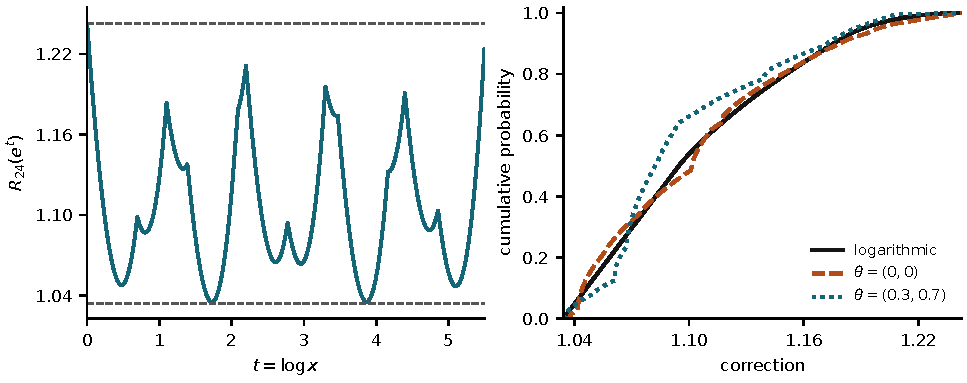
\includegraphics[width=\linewidth]{figures/laws.pdf}
\caption{The correction for $p=2$, $q=3$. Left, the solid curve is
$R_{24}(e^t)$ and the dashed lines mark its two limiting extrema.
Right, the logarithmic law and two integer subsequential laws from
\eqref{eq:natural}. Curves are deterministic quadrature approximations.}
\label{fig:laws}
\end{figure}

\section{A sharp criterion for the modulus 24}\label{sec:explicit}
For the principal character $\chi_0$ modulo $24$,
\[
 L(s,\chi_0)=\zeta(s)(1-2^{-s})(1-3^{-s}).
\]
The two extra factors have no zeros in $\Re s>0$. In particular, the
zeros in the critical strip and their multiplicities agree. The
smoothed sum gives a quantitative form of this observation. Define
\begin{equation}
 J(x)=\sum_{j\geq1}\frac{x^{-2j}}{2j(2j+1)},\qquad
 C=2+\gamma-\log(4\pi), \label{eq:J}
\end{equation}
and center the eight-spoke sum by
\[
 W_{24}(x)=E_{24}(x)-2\log x-R_{24}(x)-\log(2\pi)+J(x).
\]
\begin{theorem}\label{thm:rh}
The following statements are equivalent.
\begin{enumerate}
\item Every nontrivial zero of $\zeta$ has real part $1/2$.
\item $|W_{24}(x)|\leq C\sqrt{x}$ for every real $x\geq1$.
\item For each $\varepsilon>0$,
$E_{24}(x)=O_\varepsilon(x^{1/2+\varepsilon})$ as $x\to\infty$.
\end{enumerate}
The constant in statement 2 is forced by equality at $x=1$.
\end{theorem}
\begin{proof}
The classical smoothed explicit formula in this normalization is
\begin{equation}
 E(x)=\log(2\pi)-J(x)+
          \sum_\rho\frac{x^\rho}{\rho(1-\rho)}, \label{eq:explicit}
\end{equation}
with one term per nontrivial zero counted with multiplicity. To verify
the constants, invert the Mellin kernel $1/[s(s-1)]$ on $\Re s=2$
against $-(\zeta'/\zeta)(s)x^s$. The inverse kernel gives
$(x/n-1)_+$, including the value zero at $x=n$. Absolute convergence
permits termwise inversion. At $s=1$ the double pole contributes
$x\log x-(1+\gamma)x$. At $s=0$ the residue is
$\zeta'(0)/\zeta(0)=\log(2\pi)$, and the poles at $-2j$ contribute
$-J(x)$. The nontrivial zeros give the sum in \eqref{eq:explicit}.

For completeness, fix an integer $M\geq1$. The good-height estimate
for $\zeta'/\zeta$ gives heights $T_k\to\infty$ for which it is
$O_M(\log^2 T_k)$ uniformly on the horizontal segments from
$-2M-1$ to $2$ at heights $\pm T_k$ \cite[Lemmas 4--5]{kedlaya}.
On $\Re s=-2M-1$, the zeta functional equation and Stirling's formula
bound the logarithmic derivative by $O(\log(2+M+|\Im s|))$,
with an absolute implied constant. The odd real part keeps the
trigonometric term bounded also at height zero. The kernel contributes
$O(T_k^{-2})$ on the horizontal segments. The full integral on the
left line is $O(x^{-2M-1}\log(M+2)/(M+1))$. Taking $k\to\infty$
and then $M\to\infty$ proves \eqref{eq:explicit}.
The classical count $N(T)=O(T\log T)$ gives absolute, locally uniform
convergence of the nontrivial-zero sum for $x\geq1$.

At $x=1$, $E(1)=1+\gamma$ and
$J(1)=\sum_{j\geq1}((2j)^{-1}-(2j+1)^{-1})=1-\log2$.
Hence
\begin{equation}
 \sum_\rho\frac1{\rho(1-\rho)}=C. \label{eq:C}
\end{equation}
This classical evaluation is also recorded by Burnol \cite[p.~3]{burnol}.
Under statement 1, $\rho(1-\rho)=1/4+(\Im\rho)^2>0$ and
$|x^\rho|=\sqrt x$. By Proposition~\ref{prop:local},
$W_{24}$ is precisely the zero sum in \eqref{eq:explicit}. The
triangle inequality and \eqref{eq:C} prove statement 2, with
$W_{24}(1)=C$. Since $0\leq J(x)\leq J(1)$, the correction in
\eqref{eq:correction} is $O(1+\log x)$, so 2 implies 3.

Assume statement 3. Equation \eqref{eq:correction} transfers the same
bound to $E(x)$. Its Mellin transform
$H(s)=\int_1^\infty E(x)x^{-s-1}\dd x$ is then holomorphic on
$\Re s>1/2$, by locally uniform convergence. On $\Re s>1$, direct
integration gives
\[
 H(s)=-\frac{\zeta'(s)}{s(s-1)\zeta(s)}
             -\frac{1}{(s-1)^2}+\frac{1+\gamma}{s-1}.
\]
This identity extends meromorphically to $\Re s>1/2$. A zero
$\rho$ in the right half of the critical strip would give a pole
of the first term with residue $-\operatorname{ord}_\rho(\zeta)/
[\rho(\rho-1)]\ne0$. The other terms are regular there. Holomorphy
rules out this zero, and the functional equation rules out its
reflection in the left half of the strip. This proves statement 1.
\end{proof}
Thus an independent proof of RH by the prime-cross approach would
require an estimate for $E_{24}(x)$ in statement 3, or equivalently
the bound in statement 2. The bounded oscillation in
Theorem~\ref{thm:log} identifies exactly what removing the two Euler
factors contributes to that estimate.
\begin{cor}[A criterion on the integers]\label{cor:limsup}
With $C$ as in \eqref{eq:J},
\[
 \limsup_{n\to\infty}\frac{E_{24}(n)}{\sqrt n}=
 \begin{cases}
 C,&\text{if RH holds},\\
 +\infty,&\text{if RH fails}.
 \end{cases}
\]
In the second case the corresponding lower limit is $-\infty$.
\end{cor}
\begin{proof}
The difference $E_{24}(x)-W_{24}(x)$ is $O(1+\log x)$.
Under RH put $w_\rho=1/(1/4+(\Im\rho)^2)$. Equations
\eqref{eq:explicit} and \eqref{eq:C} give
\[
 e^{-t/2}W_{24}(e^t)=\sum_\rho w_\rho e^{it\Im\rho},
 \qquad \sum_\rho w_\rho=C.
\]
This is Nicolas's zero sum \cite[(1.18)--(1.19), Section~4]{nicolas},
whose real-argument upper limit is $C$. The recurrence argument also
applies to sampling at integers. For any finite set of ordinates and any tolerance, there are
arbitrarily large integer times $t$ at which all their phases are
within that tolerance of $1$. Indeed the phase vectors at positive
integer times have a convergent subsequence in a compact torus.
Differences of sufficiently far separated subsequence terms give the
claimed returns. Truncate the series with tail smaller than a given
$\delta>0$, and apply this argument to its finite part. Replacing
$t$ by $\log\lfloor e^t\rfloor$ changes those finitely many phases
by $o(1)$, while the absolute tail stays below $\delta$. This proves
that the upper limit along integers is $C$.

If RH fails, some zero has real part $\beta>1/2$. Suppose
$E(x)\leq K\sqrt{x}$ eventually. The Mellin transform of the
eventually nonnegative function $K\sqrt{x}-E(x)$ on $[1,\infty)$
is $K/(s-1/2)-H(s)$, initially for $\Re s>1$. Its pole at that zero
forces its abscissa of convergence $\sigma_c$ to satisfy
$\beta\leq\sigma_c\leq1$. Landau's oscillation theorem forces a
singularity at the real point $\sigma_c$ \cite[Theorem 3]{lay}.
But the formula for $H(s)$ in the preceding proof is regular on
the real interval $(1/2,\infty)$. At $1$ this follows by the
Laurent expansion $\zeta(s)=(s-1)^{-1}+\gamma+O(s-1)$, and on
$(1/2,1)$ it follows from the positive alternating eta series and
$1-2^{1-s}\ne0$. This contradiction rules out every such upper
bound. Applying the same argument to $K\sqrt{x}+E(x)$ rules out
every lower bound of the opposite sign.

To pass to integers, on $n<x<n+1$ the slope of $S_1$ is
$\sum_{j\leq n}\Lambda(j)/j=O(\log^2(2n))$, using
$\Lambda(j)\leq\log j$. The other terms of $E$ vary by
$O(\log(2n))$ across the interval. Continuity at each endpoint
gives $E(x)-E(\lfloor x\rfloor)=O(\log^2(2x))$. Together with
\eqref{eq:correction} this transfers both unbounded oscillations to
$E_{24}(n)/\sqrt n$.
\end{proof}

\section{An explicit auxiliary congruence}\label{sec:lean}
One of the conditions on an auxiliary prime in Alpöge's source is a
simultaneous congruence modulo $16$ and an odd integer $M$ \cite{source}.
It has the following explicit representative.
\begin{prop}\label{prop:crt}
For positive odd $M$ and any nonnegative integer $d$,
\[
 d\equiv7\pmod {16},\quad M\mid d+1
 \quad\Longleftrightarrow\quad d\equiv8M-1\pmod{16M}.
\]
Moreover $\gcd(8M-1,16M)=1$ for every positive integer $M$.
\end{prop}
\begin{proof}
Write $d+1=Mk$. Since $M$ is odd it acts invertibly modulo $16$
and fixes the residue $8$. Hence $Mk\equiv8\pmod{16}$ is
equivalent to $k\equiv8\pmod{16}$. This yields the claimed class,
and reversing the substitution proves the converse. Every common
divisor of $8M-1$ and $16M$ divides $16M-2(8M-1)=2$, while $8M-1$
is odd.
\end{proof}
For example $M=33$ gives $d\equiv263\pmod{528}$. With $M=3$ one
obtains $d\equiv23\pmod{48}$, which selects every other integer on
the $23$rd spoke. A prime $q>3$ with $q\equiv3\pmod8$ must lie on
the $11$th or the $19$th spoke. These congruences prescribe candidate
classes. An estimate for primes in a prescribed interval with varying
$M$ requires additional analytic input.

The accompanying Lean file proves the two spoke statements, the
explicit congruence, coprimality, and existence of the residue class.
Sections~\ref{sec:local}--\ref{sec:explicit} have mathematical proofs
in the text. The proof and verification records of Alpöge and
Sutherland concern the separate upstream project \cite{alpoge,sutherland}.

\begin{thebibliography}{10}
\bibitem{alpoge} L. Alpöge,
\emph{Announcement concerning the Riemann hypothesis},
November 20, 2026, four-page note, p.~3, item 5.
\href{https://alpo.ge/remark.pdf}{Author's note}.
\bibitem{berger} A. Berger, A note on the distributions of $(\log n)\bmod 1$,
\emph{Unif. Distrib. Theory} \textbf{17} (2022), no.~2, 77--100.
\href{https://doi.org/10.2478/udt-2022-0013}{Publisher}.
\bibitem{burnol} J.-F. Burnol, The explicit formula in simple terms,
1998, p.~3. \href{https://arxiv.org/abs/math/9810169}{arXiv:math/9810169}.
\bibitem{fgd} P. Flajolet, X. Gourdon and P. Dumas,
Mellin transforms and asymptotics: Harmonic sums,
\emph{Theoret. Comput. Sci.} \textbf{144} (1995), 3--58.
\href{https://doi.org/10.1016/0304-3975(95)00002-E}{Publisher}.
\bibitem{grant} R. E. Grant and T. Ghannam,
\emph{Philomath: The Geometric Unification of Science \& Art through
Number}, first edition, 2021, Part I, Chapter 2, The 24-Wheel and
Quasi Primes, Fig.~9 and following text.
\bibitem{kedlaya} K. S. Kedlaya, \emph{von Mangoldt's formula},
MIT 18.785, spring 2007, Lemmas 4--5 and the contour estimates.
\href{https://kskedlaya.org/18.785/von-mangoldt.pdf}{Author's notes}.
\bibitem{lay} J. P. S. Lay, Sign changes in Mertens' first and second
theorems, Theorem~3 and its application in Section~3.
\href{https://arxiv.org/abs/1505.03589}{arXiv:1505.03589}.
\bibitem{nicolas} J.-L. Nicolas, Small values of the Euler function and
the Riemann hypothesis, 2012, (1.18)--(1.19) and Section~4.
\href{https://arxiv.org/abs/1202.0729}{arXiv:1202.0729}.
\bibitem{plichta} P. Plichta, lecture at the Technische Universität
Ilmenau, June 7, 2005, description of the \emph{Primzahlkreuz}.
\href{https://www.plichta.de/plichta/vortrag-in-illmenau/gehalten-an-der-uni-illmenau-am-7-6-05}{Lecture text}.
\bibitem{source} L. Alpöge, Lean source accompanying \cite{alpoge},
\texttt{chineseRemainder\_finiteCover}, module
\texttt{ExistsCoprimePrimePairSetSecondEqPPset}.
\href{https://github.com/Deicyde/riemann-hypothesis/blob/371a1a26d5e17f604428e3a8ce6ce341cf517434/src/Development/AutomorphicArithmetic/MeanSquareBounds/ExistsCoprimePrimePairSetSecondEqPPset.lean}{Pinned copy of the source}.
\bibitem{sutherland} A. V. Sutherland,
\emph{Verification files for the Lean proof of the Riemann Hypothesis},
status dated November 20, 2026, 22:05 UTC.
\href{https://math.mit.edu/~drew/grh/}{Verification records}.
\bibitem{weyl} H. Weyl, \"Uber die Gleichverteilung von Zahlen mod.
Eins, \emph{Math. Ann.} \textbf{77} (1916), 313--352.
\href{https://doi.org/10.1007/BF01475864}{Publisher}.
\bibitem{xu} C. Xu, The distributional asymptotics mod 1 of
$(\log_b n)$, \emph{Unif. Distrib. Theory} \textbf{14} (2019),
no.~1, 105--122.
\href{https://doi.org/10.2478/udt-2019-0007}{Publisher}.
\end{thebibliography}

\end{document}
